%%%%%%%%%%%%%%%%%%%%%%%%%%%%%%%%%%%%%%%%%
% Arsclassica Article
% LaTeX Template
% Version 1.0 (21/4/14)
%
% Original author:
% Lorenzo Pantieri (http://www.lorenzopantieri.net) with extensive modifications by:
% Vel (vel@latextemplates.com)
%
% License:
% CC BY-NC-SA 3.0 (http://creativecommons.org/licenses/by-nc-sa/3.0/)
%%%%%%%%%%%%%%%%%%%%%%%%%%%%%%%%%%%%%%%%%

%----------------------------------------------------------------------------------------
%	PACKAGES AND OTHER DOCUMENT CONFIGURATIONS
%----------------------------------------------------------------------------------------

\documentclass[
10pt, % Main document font size
a4paper,
oneside, % One page layout (no page indentation)
%twoside, % Two page layout (page indentation for binding and different headers)
headinclude,footinclude, % Extra spacing for the header and footer
BCOR5mm, % Binding correction
]{scrreprt}

%%%%%%%%%%%%%%%%%%%%%%%%%%%%%%%%%%%%%%%%%
% Arsclassica Article
% Structure Specification File
%
% Original author:
% Lorenzo Pantieri (http://www.lorenzopantieri.net) with extensive modifications by:
% Vel (vel@latextemplates.com)
%
% License:
% CC BY-NC-SA 3.0 (http://creativecommons.org/licenses/by-nc-sa/3.0/)
%%%%%%%%%%%%%%%%%%%%%%%%%%%%%%%%%%%%%%%%%

%----------------------------------------------------------------------------------------
%	REQUIRED PACKAGES
%----------------------------------------------------------------------------------------
\usepackage[
nochapters, % Turn off chapters since this is an article        
beramono, % Use the Bera Mono font for monospaced text (\texttt)
eulermath,% Use the Euler font for mathematics
pdfspacing, % Makes use of pdftex’ letter spacing capabilities via the microtype package
dottedtoc % Dotted lines leading to the page numbers in the table of contents
]{classicthesis} % The layout is based on the Classic Thesis style

\usepackage{arsclassica} % Modifies the Classic Thesis package

\usepackage[T1]{fontenc} % Use 8-bit encoding that has 256 glyphs

\usepackage[french]{babel}

\usepackage[utf8]{inputenc} % Required for including letters with accents

\usepackage{graphicx} % Required for including images

\graphicspath{{figures/}} % Set the default folder for images

\usepackage{enumitem} % Required for manipulating the whitespace between and within lists

\usepackage{lipsum} % Used for inserting dummy 'Lorem ipsum' text into the template

\usepackage{subfig} % Required for creating figures with multiple parts (subfigures)

\usepackage{amsmath,amssymb,amsthm} % For including math equations, theorems, symbols, etc

\usepackage[french]{varioref} % More descriptive referencing

\usepackage{verbatimbox} % Centered verbatim
\usepackage{algorithm2e}
%----------------------------------------------------------------------------------------
%	THEOREM STYLES
%---------------------------------------------------------------------------------------
\theoremstyle{definition} % Define theorem styles here based on the definition style (used for definitions and examples)
\newtheorem{definition}{Definition}

\theoremstyle{plain} % Define theorem styles here based on the plain style (used for theorems, lemmas, propositions)
\newtheorem{theorem}{Theorem}

\theoremstyle{remark} % Define theorem styles here based on the remark style (used for remarks and notes)

%----------------------------------------------------------------------------------------
%	HYPERLINKS
%---------------------------------------------------------------------------------------
\hypersetup{
%draft, % Uncomment to remove all links (useful for printing in black and white)
colorlinks=true, breaklinks=true, bookmarks=true,bookmarksnumbered,
urlcolor=webbrown, linkcolor=RoyalBlue, citecolor=webgreen, % Link colors
pdftitle={}, % PDF title
pdfauthor={\textcopyright}, % PDF Author
pdfsubject={}, % PDF Subject
pdfkeywords={}, % PDF Keywords
pdfcreator={pdfLaTeX}, % PDF Creator
pdfproducer={LaTeX with hyperref and ClassicThesis} % PDF producer
} % Include the structure.tex

\hyphenation{Fortran hy-phen-ation}

%----------------------------------------------------------------------------------------
%	TITLE AND AUTHOR(S)
%----------------------------------------------------------------------------------------
\title{Vector Racer}
\title{\normalfont\spacedallcaps{Vector Racer}}

\date{}

%----------------------------------------------------------------------------------------

\begin{document}

%----------------------------------------------------------------------------------------
%	HEADERS
%----------------------------------------------------------------------------------------

\renewcommand{\sectionmark}[1]{\markright{\spacedlowsmallcaps{#1}}} % The header for all pages
%\renewcommand{\subsectionmark}[1]{\markright{\thesubsection~#1}} % this modifies the header on odd pages
\lehead{\mbox{\llap{\small\thepage\kern1em\color{halfgray} \vline}\color{halfgray}\hspace{0.5em}\rightmark\hfil}}

\pagestyle{scrheadings}

%----------------------------------------------------------------------------------------
%	TABLE OF CONTENTS & LISTS OF FIGURES AND TABLES
%----------------------------------------------------------------------------------------

\maketitle

\setcounter{tocdepth}{2}

\tableofcontents

\listoffigures

\listoftables

\newpage

%----------------------------------------------------------------------------------------
%	INTRODUCTION
%----------------------------------------------------------------------------------------
\section*{Introduction}
\textit{Vector Racer} est originellement un jeu de course de voitures, que l'on peut déplacer sur des cases d'une grille. Le jeu gère les notions de vitesses et d'accélération des voitures, si bien qu'il devient difficile de tourner rapidement avec une vitesse trop élevée. L'objectif de ce jeu est d'arriver en tête de la course tout en évitant les obstacles comme les murs par exemple.

Comme toute course, le joueur cherchera à minimiser son temps de parcours et de fait, à maximiser la vitesse tout en minimisant la distance parcourue. On comprend déjà que notre algorithme de résolution va chercher un parcours qui va correspondre en tout point à une optimisation à la fois de la distance parcourue et de la vitesse.

Nous allons donc poser dans un premier temps les problèmes à résoudre ainsi que le vocabulaire que nous allons employer pour caractériser le jeu. Nous verrons ensuite comment nous avons implémenté les types abstraits de données qui apparaissent dans les problèmes évoqués ci-dessus puis nous terminerons par présenter l'algorithme de résolution et l'ensemble des tests réalisés pour vérifier sa validité.

\subsection*{Capacité du programme réalisé}

Notre programme permet d'afficher, de jouer et de résoudre une carte donnée en paramètre.
La résolution de la carte n'est pas une résolution optimale. Il s'agit d'une solution non triviale de parcours du circuit.

%----------------------------------------------------------------------------------------

\newpage

%----------------------------------------------------------------------------------------
%	ALGORITHMIQUE DU JEU
%----------------------------------------------------------------------------------------
\chapter{Algorithmique du jeu}

%----------------------------------------------------------------------------------------
%	DÉFINITIONS
%----------------------------------------------------------------------------------------
\section{Définitions}
Les mots que nous allons utiliser pour décrire un objet ou un concept précis mis en oeuvre dans la résolution du problème sont des mots pouvant donner lieu à de nombreuses lectures et approches différentes qui peuvent fausser les démonstrations qui s'appuient dessus. Pour fixer les idées, nous nous devons d'imposer des bases, seul appui pour nos raisonnements ultérieurs.

\subsection{Cartes}
\label{ssect:cartes}

Une \textit{case} $c$ sera considérée comme un élément admettant plusieurs états possibles, représentés par les cas suivants :
\begin{itemize}
\item une case associée au symbole $\star$ représente une position de départ possible pour la course,
\item une case associée à un entier de 0 à 9 fait partie de la piste du circuit, et est donc la zone parcourable par les voitures,
\item une case est enfin associée au symbole $\#$ lorsqu'elle représente un obstacle (mur bordant la piste par exemple), qui n'est pas accessible au voitures.
\end{itemize}

Une \textit{carte} $\mathcal{C}$ (c.f. exemple Figure~\vref{fig:ex_carte}) est une structure contenant des cases, organisées sous forme d'une matrice de dimension $n\times m$, et sur laquelle est définie une fonction $\eta_\mathcal{C}$ à valeur dans l'ensemble $\Omega = \{\star, \#, [1-9]\}$ telle que $\forall c\in \mathcal{C}, \exists \omega\in \Omega, \eta_\mathcal{C} = \omega$. Cette fonction permet donc d'accéder à l'état d'une case.

Un case sera dite \textit{valide} si son état est dans l'ensemble $\Omega_V = \{\star, [1-9]\}$.

On défini la notion de \textit{chemin} sur la carte comme une séquence de cases - donc de positions - prises par un véhicule. Un \textit{parcours} est un chemin partant et aboutissant dans une case étiquetée par $\star$. Un parcours est dit \textit{valide} si et seulement si les cases sont parcourue dans l'ordre croissant depuis la position de départ, à partir d'une case étiquetée par 1 et que les coups élémentaires sont valides (voir Section~\vref{ssect:coups}). Enfin, un parcours est \textit{complet} - appelé aussi \textit{tour} - si il est valide et que l'ensemble des positions élémentaires fait apparaitre au moins une fois chaque chiffre visible sur la carte. La position d'arrivé est soit une case étiquetée par $\star$, soit une case étiquetée par $1$.

Notons qu'une carte est \textit{valide} si et seulement si elle respecte les contraintes suivantes :
\begin{enumerate}
\item elle comporte au moins une case à l'état $\star$,
\item l'ensemble formé par les cases d'étiquette dans $\Omega_V$ est connexe,
\item il existe au moins un tour.
\end{enumerate}

\begin{verbbox}
#######
#33332#
#4###2#
#4###2#
#*1111#
#######
\end{verbbox}
\begin{figure}[ht]
	\centering
	\theverbbox
	\caption{Exemple de carte $7\times 6$}
	\label{fig:ex_carte}
\end{figure}

\subsection{Coups}
\label{ssect:coups}

Le jeu \textit{Vector Racer} présente des règles particulières quant aux coups possibles à chaque étape, du fait de la considération de la vitesse et de l'accélération du véhicule. Le principe général est le suivant :
\begin{enumerate}
\item on considère le vecteur vitesse du véhicule à chaque étape : $\begin{pmatrix}x\\y\end{pmatrix}$ (composantes dans le repère orthonormé direct associé à la grille),
\item étant donné une séquence d'accélérations possibles (dépendantes des performances du véhicule), par exemple $\begin{pmatrix}dx\\dy\end{pmatrix}$, le vecteur vitesse à l'étape suivante est $\begin{pmatrix}x+dx\\y+dy\end{pmatrix}$.
\end{enumerate}

Ce vecteur vitesse et la séquence des accélérations possibles conditionnent ainsi l'accès à certaines cases à chaque étape.

Un coup est \textit{valide} si et seulement si :
\begin{enumerate}
\item les positions de départ et d'arrivée sont valides sur la grille (c.f. Section~\vref{ssect:cartes}),
\item la variation du vecteur vitesse induite par ce coup correspond à une accélération possible (parmis celle de la séquence d'accélérations que l'on considère).
\end{enumerate}

\begin{table}[ht]
	\centering
	\begin{tabular}{| c || c | c | c |}
	\hline
	Accélérations possibles & Coups effectuées & Variation de vitesse & Case \\ \hline
	1,1 & &  & $\star$ \\ \hline
	-1,-1 & 1,0 & 1,0 & 1 \\ \hline
	-1,0 & 2,0 & 1,0 & 1 \\ \hline
	-1,1 & 1,1 & -1,1 & 1 \\ \hline
	0,-1 & 0,1 & -1,0 & 2 \\ \hline
	0,0 & -1,1 & -1,0 & 2 \\ \hline
	0,1 & -2,0 & -1,-1 & 2 \\ \hline
	1,-1 & -1,-1 & 1,-1 & 3 \\ \hline
	1,0 & 0,-1 & 1,0 & 3 \\ \hline
	& 0,-1 & 0,0 & 4 \\ \hline
	& 1,0 & 1,1 & $\star$ \\
	\hline
	\end{tabular}
	\caption{Exemple de liste de coups possibles pour la carte Figure~\vref{fig:ex_carte}}
	\label{tab:ex_coups}
\end{table}

\newpage

%----------------------------------------------------------------------------------------
%	PROBLÈMES
%----------------------------------------------------------------------------------------
\section{Problèmes}
\subsection{Spécifications}

\begin{verbatim}
Problème : Résolution
Entrée : Une grille G représentant la carte réalisable.
Sortie : Une liste de coups valide.
\end{verbatim}



\section{Résolution}
\subsection{Choix de l'algorithme}
Le but du jeu Vector Racer est de trouver le plus court chemin faisant le parcours d'une grille. Les notions de chemins et parcours nous ont poussés à considérer plusieurs algorithmes connues sur les graphes susceptibles de résoudre ce problème. Il s'agit en effet du parcours en largeur, du parcours en profondeur, de Dijkstra et de A*. Ces algorithmes garantissent tous des solutions, néamoins ils sont plus ou moins optimales. Le parcours en profondeur par exemple ne renvoie pas le plus court chemin. A* quand à lui nécessite des heuristiques très difficles à généraliser vu le grand nombre de cartes possibles. Dijkstra et le parcours en largeur à l'opposée semblent très adéquats au problème, ce sont d'ailleurs les deux algorithmes que nous avons choisis d'implémenter pour chercher les solutions.

En effet, ces deux algorithmes évoluent progressivement vers la solution en minimisant le nombre de coups. Dans le cas du jeu Vector Racer, la connaissance seulement de la position et la vitesse permet à chaque étape de générer un ordre convenable de successeurs, vers lequels le joueur peut se déplacer en maximisant sa vitesse tout en se rapprochant de la destination. Dans la section qui suit, nous allons présenter l'implémentation de l'algorithme de résolution. Nous allons aussi détailler quelques fonctions auxiliaires essentielles dans la prise de décision. \\

\begin{algorithm}[H]
 \KwData{carte}
 \KwResult{solution}
 f $\leftarrow$ file-vide()\;
 Enfiler le noeud position de départ\;
 \While{no-vide(f)}{
  Défiler\;
  Colorer le noeud\;
  Générer les 8 successeurs possibles\;
  Parmis ces successeurs, choisir ceux qui maximisent l'accélération\;
  Chaîner les successeurs séléctionnés au noeud coloré\;
  	\For{Chaque successeur}{
		\eIf{Le successeur est le noeud d'arrivée}{
			Retourner le noeud\;
			}
			{
			Enfiler le noeud\;
			}	
	}
   
  
 }
 \caption{Algorithme de résolution d'une grille}
\end{algorithm}

%------------------------------------------------------------------------------
%   REALISATION
%------------------------------------------------------------------------------

\chapter{Réalisation du programme}
\section{Structures de données}
	
Certaines des structures de données ne sont utilisées que par certains modules du programme. Il n'est donc pas nécessaire de les abstraire. En revanche, certaines de ces structures sont utilisées par plusieurs modules, c'est le cas de la liste chaînée.
	\subsection{Structures simples}
    
	\subsubsection{La structure map}
    La structure map est construite par le parseur de cartes, contenu dans le module de parsing.
	les champs de cette structure sont :
	\begin{itemize}
		\item Un entier hauteur
		\item Un entier largeur
		\item Un tableau de caractères
		\item Une structure position pour repérer le point de départ
		\item Un entier pour le maximum de checkpoints
	\end{itemize}	
    
	\subsubsection{La structure steps}
	La structure steps est un ensemble de coups relatifs à une carte. Elle est générée par le parseur de coups. Elle peut être utilisée,par exemple, pour de comparer les performences d'autres intelligences artificelles.\\
Elle contient : 
	\begin{itemize}
		\item Un entier pour le nombre d'accélérations
		\item Un entier pour le nombre d'étapes
		\item Une structure point pour la position de départ
		\item Deux tableaux de structures point contenant les positions et vitesses correspondantes
	\end{itemize}	
	\subsubsection{La structure point}
    Cette structure est exclusivement utilisée par les modules de moteur de jeu, ainsi que l'affichage graphique. \\
	La structure point est une structure simple à deux champs entiers. Ces deux nombres représentent une position sur la grille. Le moteur de jeu utilise cette structure pour communiquer une position à l'interface.\\
	
	\subsubsection{La structure node}
    La structure node est utilisée par le module de résolution d'une carte. Elle contient quatre champs entiers, correspondants à une position et une vitesse. Elle contient de plus un champs pointeur sur le noeud précédent.\\

Grâce à l'abscence de typage des données dans la liste chaînée (pointeur void), nous pouvons stocker des données de n'importe quel type dans une liste chaînée, notemment les structures point (pour le moteur de jeu) et node (pour le solveur).



	\subsection{Structures abstraites}	
    La seule structure ayant été sujet d'une abstraction est la liste chaînée.
	\subsubsection{Mise en oeuvre}
	Le type de données utilisée içi est une liste doublement chainée	
	\begin{figure}[h]
	\centering
	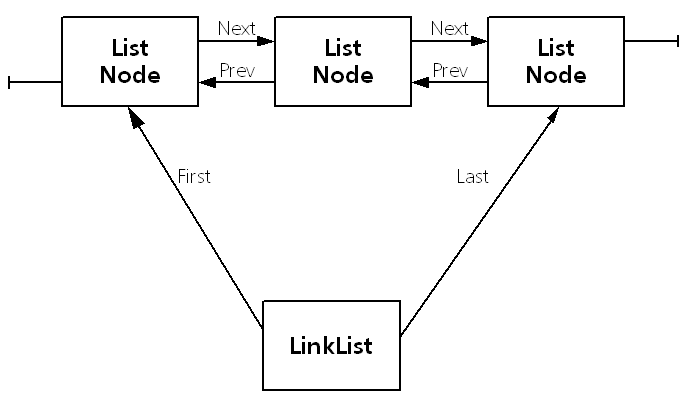
\includegraphics[scale = 0.3]{linklist.png}
    \caption{Double linked list}
    \end{figure} \\
    Les structures sont donc: \\
	\texttt{liste}
	\begin{itemize}
	\item pointeur sur l'élément tête
	\item pointeur sur l'élément queue
	\item entier nombre d'éléments (à 0 initialement)
	\end{itemize}
	\texttt{element}
    \begin{itemize}
	\item pointeur sans type sur une donnée
	\item pointeur élément sur l'élément précédent
	\item pointeur élément sur l'élément suivant
	\end{itemize}
	\subsubsection{Primitives}
  	Les primitives utilisées pour gérer la liste sont les suivantes : \\
	\texttt{list\_empty} qui teste si la liste est vide. \\
    \texttt{list\_head} renvoie la tête de la liste.\\
	\texttt{list\_tail} renvoie la queue de la liste. \\
    Celles relatives aux éléments sont :
	\texttt{list\_data} qui renvoie un pointeur sans type sur le champ donné de l'élément passé en paramètre.\\	
	\texttt{list\_next} renvoie le pointeur sur l'élément suivant. \\
	\texttt{list\_previous} renvoie le pointeur sur l'élément précédent. \\

	\subsubsection{Intérêt}
	L'abstraction de la liste chainée et de ses élements la rend utilisable par n'importe module sans qu'il n'ai connaissance de son implémentation. Cela permet notemmment de l'utiliser pour lister des coups jouables avec le solveur, ou de générer une liste de positions jouées. \\

	Le double chaînage permet de réduire la complexité de la fonction \texttt{list\_add} (qui effectue un ajout en queue). Avec une liste simple elle aurait été $\theta(n)$ en la taille de la liste, içi elle est en $\theta(1)$. De même pour la fonction de retrait en queue.\\








































\section{Le module SDL}

Un jeu pour qu'il en soit un a besoin d'une interface. Cette interface est indispensable pour le joueur. Sans elle il n'y aurait pas d'échange d'information entre l'utilisateur et la machine.

Nous avons fait le choix d'utiliser la bibliothèque SDL pour réaliser l'interface de vector racer. L'avantage de cette bibliothèque est qu'elle permet à la fois une gestion de l'affichage,du temps et des évènements (principalement les choix de l'utilisateur). Nous avions de plus  de l'expérience avec cette bibliothèque, ce qui a facilité notre choix.

Lien pour la bibliothèque SDL: http://www.libsdl.org

Les fonctions utilisant directement la SDL sont regroupées dans le module vectorSDL. A l'exception du module vectorGame, aucun autre module ne touche directement aux fonctions de la bibliothèque SDL. Nous avons fait ce choix afin de simplifier son utilisation.

\section{Moteur de jeu}

Le joueur va parcourir le circuit et traverser les différentes zones. Les évènements (les choix de l'utilisateur) sont traités grâce à des fonctions de la bibliothèque SDL.
Pour déterminer si le joueur perd,gagne ou triche, il faut que l'on vérifie à chaque étape la situation du joueur.

La première situation à vérifier est la colision avec un mur. On vérifie donc que le joueur ne tombe pas sur une case mur.
Nous n'avons pas traité le fait qu'un tracé peut traverser un mur sans s'y arrêter.

La deuxième situation est la fin du circuit. Pour gérer l'évènement, on considère le circuit comme terminé si le joueur est bien passé par toute les zones de checkpoint et qu'il est revenu soit sur la case départ, soit sur un checkpoint inférieur en valeur aux deux dernier checkpoint.

Enfin, il faut vérifier que le joueur ne rate pas un checkpoint. Pour cela on crée un compteur qui vérifie que la valeur du dernier checkpoint atteint augmente bien de manière régulière (sans sauts). 

\section{Mise en oeuvre de l'algorithme de résolution}
\subsection{Implémentation}
Nous avons implémenté l'algorithme de recherche en largeur en utilisant une structure noeud (cf. FIgure~\ref{noeud}). Cette structure contient 4 entiers représentant la position dans la grille et la vitesse en cette position. De plus elle contient un pointeur sur un noeud qui va servir à retracer le chemin qui a généré ce noeud.

\begin{figure}[h]
\centering
\begin{minipage}[c]{0.5\linewidth}
\begin{verbatim}
Struct node{
int x,y,dx,dy;
struct node * parent;
}
\end{verbatim}
\end{minipage}
\caption{Définition de struct noeud}
\label{noeud}
\end{figure}
Pour stocker ces noeud nous utilisons une structure liste. L'algorithme manipule deux listes pricipales : "queue" et "colored" en plus d'une liste temporaire "successors". La liste "queue" sert à stocker les noeuds 'candidats' qui potentiellement font avancer le chemin le plus vers la destination. "colored" quand à elle sert à mémoriser les noeuds déjà essayés. "successors" est une liste qui stocke temporairement tous les successeurs de la position courante.

Au début de l'algorithme, la liste "queue" contient uniquement la position de départ correspondant à une '*' dans la grille. Une fonction "generate-successors" s'occupe de générer les noeuds successeurs de cette position, il y'en a au maximum neuf, correspondant aux neuf accélérations possibles. Ces noeud successeurs sont générés dans l'ordre faisant maximiser la norme de la vitesse. Dans ce sens où le noeud de norme la plus grande est généré à la fin. Ensuite les champs parents de ces successeurs pointeront sur le noeud qui les a générés (le noeud source). Pour chacun de ces successeurs, l'algorithme va tester si sa position corrspond à une position destination. Si ce n'est pas le cas et qu'il n'a pas déjà été visité, il sera ajouté à "queue". L'étape suivante consiste à rajouter le noeud source à "colored" et continuer la recherche à partir du dernier élément de "queue". Ce processus sera répété jusqu'à ce que l'algorithme tombe sur un noeud destination et que le chemin parcouru soit valide, ou alors la liste "queue" devienne vide. 

Pour décider de la validité du chemin parcouru, une fonction "valid-path" a été implémenté. Elle retrace les neouds parcourues grâce au champs parent, et vérifie que le chemin passe par toutes les zones dans l'ordre croissant. Elle vérifie aussi si toutes les positions sont valides dans la grille. Par contre elle ne vérifie pas le fait que l'on puisse sauter sur des obstacles.

D'autres fonctions auxiliaires, mais très importantes, ont été impléméntés. Notamment "identify-zones" qui identifie les zones d'une map et "order-of-accelerations" qui ordonne les accélérations selon la norme.
\subsection{Tests et performances}

Nous avons testé notre algorithme sur plusieurs grilles de tailles différentes. La Figure~\ref{solution} montre un exemple de résolution sur une carte de taille 30x30. La liaison avec le module SDL permet de visualiser la validité de la solution proposée par l'algorithme, cependant nous ne disposons d'aucune outil permettant de confirmer l'optimisation.

Généralement, notre solveur propose des solutions instantanée pour des grilles d'ordre inférieur à 100x100. Il faut présiser que notre solver ne vérifie pas si une grille est valide avant de la résoudre.

Nous avons aussi envisgé de tester toutes les parties de notre algorithme. Ou à la limite ses fonctions pricipales. Mais la réalisations de ses tests s'est avérée insuffisante pour en tier des conclusions, puisque nous nous sommes basés sur des cas très particuliers qui ne peuvent être généralisés.
\begin{figure}[h]
\centering 
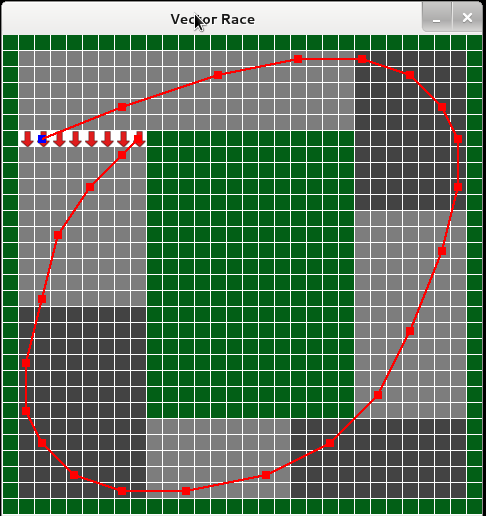
\includegraphics[scale=0.5]{Capture_du_2014-05-27_22-22-04.png}
\caption{Exemple de résolution}\label{solution}
\end{figure}

%------------------------------------------------------------------------------
%   REMARQUE ET AMELIORATION POSSIBLES
%------------------------------------------------------------------------------
\chapter{Remarques et améliorations possibles}

\section{Fuites mémoire}

Malheureusement il reste des fuites mémoire.

La plupart sont dûes à la SDL. Valgrind indique que des allocations de la fonction SDL\_Init() n'ont pas été libérées. Notre connaissance de SDL n'étant pas parfaite nous ne savons pas comment régler ces fuites mémoires.

Il reste cependant des fuites mémoires qui correspondent à la libération de la structure map et à la libération de structures dans le solveur.
Nous n'avons pu régler ce problème avant la limite de temps malgrès nos tentative de correction. C'est donc un travail qu'il reste à faire.

\section{Idées supplémentaires}

De nombreuses possibilités d'amélioration existent.
En voici quelques unes:
\begin{itemize}
	\item L'optimisation de la résolution.
	\item La possibilité en jouant de revenir en arrière sur les choix effectués.
    \item L'affichage de la solution en parallèle de la phase de jeu.
\end{itemize}
\end{document}
